\documentclass[12pt,a4paper]{article}
\usepackage[utf8]{inputenc}
\usepackage{amsmath}
\usepackage{amsfonts}
\usepackage{amssymb}
\usepackage{makeidx}
\usepackage{graphicx}
\usepackage[left=2cm,right=2cm,top=2cm,bottom=2cm]{geometry}

\begin{document}
\title{\textbf{Sistemas electronicos de interfaz\\EV 2.4. Giro de un motor en corriente directa\\Tarea 4}}
\author{Josue Natanael Orozco Nevares 18311797\\Ing. Mecatronica\\Grado 4B}
\date{15 de octubre del 2019}
\maketitle
\begin{figure}[h!]
\centering

\includegraphics[width=9cm]{UPCDLZMDG5783-logo.png} 
\end{figure}
\newpage

\section{Introducciòn}
En esta investigaciòn descubriremos el funcionamiento adecuado cuando hacemos girar un motor cuando es de corriente directa, indagando en los porques y su mecanismo.

\section{Motor de corriente directa}
Los motores de Corriente Directa o motor DC(correspondiente a las iniciales en inglés “direct current”) es también conocidos como motor de Corriente Continua o motor CC, son  muy utilizados en diseños de ingeniería debido a las características torque-velocidad que poseen con diferentes configuraciones eléctricas o mecánicas.\\
Una gran ventaja de los motores de CD se debe a que es posible controlarlos con suavidad y en la mayoría de los casos son reversibles, responden rápidamente gracias a que cuentan con una gran razón de torque a la inercia del rotor. Otra ventaja es la implementación del frenado dinámico, donde la energía generada por el motor se alimenta a un resistor disipador, y el frenado regenerativo donde la energía generada por el motor retroalimenta al suministro de potencia CD, esto es muy utilizado en aplicaciones donde se deseen frenados rápidos y de gran eficiencia.
\begin{figure}[h!]
\centering
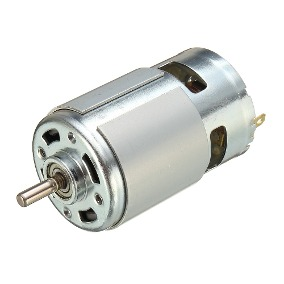
\includegraphics[width=5cm]{775-corriente-continua-12v-36v-3500-9000rpm-motor-bola-tenie-D_NQ_NP_791793-MLM31405059472_072019-Q.jpg} 
\end{figure}

\section{Fundamentos de las maquinas de corriente continua}
Las máquinas de corriente contínua son generadores que convierten energía mecánica en energía eléctrica de corriente continua, y motores que convierten energía eléctrica de corriente continua en energía mecánica. La mayoría las máquinas de corriente contínua son semejantes a las máquinas de corriente alterna ya que en su interior tienen corrientes y voltajes de corriente alterna. Las máquinas de corriente contínua tienen corriente contínua sólo en su circuito exterior debido a la existencia de un mecanismo que convierte los voltajes internos de corriente alterna en voltajes corriente continua en los terminales. Este mecanismo se llama colector, y por ello las máquinas de corriente continua se conocen también como máquinas con colector.
\newpage

\section{Funcionamiento de motor de corriente directa}
El principio de funcionamiento de los motores eléctricos de corriente directa o continua se basa en la repulsión que ejercen los polos magnéticos de un imán permanente cuando, de acuerdo con la Ley de Lorentz, interactúan con los polos magnéticos de un electroimán que se encuentra montado en un eje. Este electroimán se denomina “rotor” y su eje le permite girar libremente entre los polos magnéticos norte y sur del imán permanente situado dentro de la carcasa o cuerpo del motor.


\end{document}